\documentclass[tikz,border=5mm]{standalone}
\usepackage{tikz}
\usetikzlibrary{calc,angles}

\begin{document}
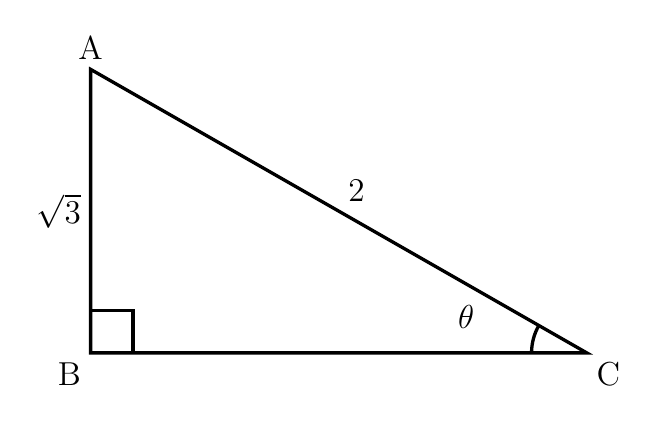
\begin{tikzpicture}[scale=1.8]

% Define vertices
\coordinate (A) at (0,2);
\coordinate (B) at (0,0);
\coordinate (C) at (3.5,0);

% Draw triangle ABC
\draw[very thick] (A) -- (B) -- (C) -- cycle;

% Draw right angle mark at B
\draw[very thick] (B) ++(0.3,0) -- ++(0,0.3) -- ++(-0.3,0);

% Angle arc at C (θ) - inside the triangle using angles library
\pic[draw, very thick, angle radius=7mm] {angle=A--C--B};
\node at ($(C)+(-0.85,0.25)$) {\large $\theta$};

% Vertex labels
\node[above] at (A) {\large A};
\node[below left] at (B) {\large B};
\node[below right] at (C) {\large C};

% Side labels
\node[left] at ($(A)!0.5!(B)$) {\large $\sqrt{3}$};
\node[above right] at ($(A)!0.5!(C)$) {\large $2$};

\end{tikzpicture}
\end{document}